\documentclass[11pt,spanish]{article} % Tipo y tamaño de letra del documento.


\usepackage[utf8]{inputenc}
\usepackage{subfiles}
\usepackage{biblatex}
\addbibresource{references.bib}
\usepackage{multicol}
\usepackage{amsfonts}
\usepackage{blindtext}
\usepackage{mathrsfs}
\usepackage{amsmath}
\usepackage{siunitx}
\usepackage{centernot}
\usepackage[shortlabels]{enumitem}
\usepackage{subfig}
\usepackage{datetime}
\usepackage{listingsutf8}
\usepackage[spanish]{babel}
\usepackage{tikz}
\usepackage{hyperref}
\usepackage[vlined,ruled,linesnumbered]{algorithm2e}
\usepackage{listings}
\usepackage{float}
\usepackage{url}
\usepackage{csquotes}
\usepackage{fourier} %font
\usepackage[top=2cm, bottom=2cm, left=2.5cm, right=2.5cm]{geometry}
\usepackage{pgfplots}
\usepackage{fancyhdr}
\usepackage{mdframed}
\usepackage{tikzducks}
\usepackage[nameinlink]{cleveref}
\usepackage{epigraph} 

\pgfplotsset{compat=1.18}

\usetikzlibrary{shapes.arrows, shapes.geometric, arrows.meta,angles,quotes,positioning,arrows,fit,quotes,calc}
\tikzset{>=latex} 

\setlength\algomargin{1em} 
\SetFuncSty{sc} 
\SetCommentSty{em} 


\Crefname{figure}{Fig.}{Figs.}
\newcommand\crefrangeconjunction{--}
\Crefname{table}{Tabla}{Tablas}
\Crefname{subsubsection}{Subsubsec.}{Subsubsections}
\Crefname{subsection}{Subsec.}{Subsections}
\Crefname{section}{Sec.}{Sections}
\Crefname{equation}{eq.}{eqs.}
\crefname{thm}{Theorem}{theorems}
\Crefname{thm}{Theorem}{Theorems} 

\definecolor{algoco}{rgb}{0,0.4,1}

\hypersetup{
  colorlinks=true,
  linkcolor=algoco,
  citecolor=blue,
  urlcolor=blue,
}

\lstset{
extendedchars=true
inputencoding=utf8/latin1,
basicstyle=\footnotesize\sffamily\color{black},
commentstyle=\slshape \color{gray},
numbers=left,
numbersep=10pt,
numberstyle=\tiny\color{red!80!black},
keywordstyle=\color{red!80!magenta},
showspaces=false,
showstringspaces=false,
stringstyle=\color{cyan!80!black},
tabsize=2,
literate={á}{{\'a}}1 {é}{{\'e}}1 {í}{{\'i}}1 {ó}{{\'o}}1 {ú}{{\'u}}1,
frame = single, 
numbers = none,
float, floatplacement = ht, captionpos = b,
xleftmargin = 2em, xrightmargin = 2em, 
}

\newcommand{\ub}[1]{\underbrace{#1}}
\newcommand\tcm{\textcolor{magenta}}
\newcommand\tca{\textcolor{algoco}}

\setlength\epigraphwidth{.7\textwidth} 

\newcommand{\tnum}{2 y 3} % reemplace 2 por el número de la tarea
\newcommand{\sem}{2024-2} % reemplace 2024-2 por el semestre correspondiente
\newcommand{\campus}{San Joaquín \\ Santiago} % reemplace Casa Central por el campus correspondiente
\newcommand{\rolusm}{202073628-6} % reemplace 2025073100-1 por su rol
\newcommand{\namestudent}{Luis Zegarra Stuardo} % reemplace Al Goritmo Pérez por su nombre

\headheight=14pt
\linespread{1.3}
\author{\namestudent}
\pagestyle{fancy}
\fancyhf{}%
\fancyfoot[R]{ \namestudent \\ \rolusm}
\fancyfoot[L]{Campus \campus} 
\fancyfoot[C]{\thepage}
\rhead{2024-2}
\lhead{INF-221}
\renewcommand{\headrulewidth}{0.4pt}
\renewcommand{\footrulewidth}{0.4pt}
\newbool{programs}
\boolfalse{programs}
\chead{REPORTE TAREA \tnum~}



\title{
  \huge
  \textbf{REPORTE TAREA \tnum~ \\ ALGORITMOS Y COMPLEJIDAD} \\[1ex]
  \emph{\textquote{Explorando la Distancia entre Cadenas, una Operación a la Vez}}
  }

  
\date{
  \small
  \today\\
  \currenttime
}




\begin{document}
\maketitle
\thispagestyle{fancy} 
\vspace{-1.0\baselineskip}




\begin{abstract}
  \textit{ 
    Un resumen es un breve compendio que sintetiza todas las secciones clave de un trabajo de investigación: la introducción, los objetivos, la infraestructura y métodos, los resultados y la conclusión. Su objetivo es ofrecer una visión general del estudio, destacando la novedad o relevancia del mismo, y en algunos casos, plantear preguntas para futuras investigaciones. El resumen debe cubrir todos los aspectos importantes del estudio para que el lector pueda decidir rápidamente si el artículo es de su interés.

En términos simples, el resumen es como el menú de un restaurante que ofrece una descripción general de todos los platos disponibles. Al leerlo, el lector puede hacerse una idea de lo que el trabajo de investigación tiene para ofrecer \cite{elsevier_abstract_2024}.

\textbf{La extensión del resumen, para esta entrega, debe ser tal que la totalidad del índice siga apareciendo en la primera página. Recuerde que NO puede modificar el tamaño de letra, interlineado, márgenes, etc.}

  }
     
\end{abstract}

\setcounter{tocdepth}{1}
\tableofcontents


\newpage
\section{Introducción}
Hoy en día, en la era de la tecnología, la \textbf{calidad y eficiencia de los programas computacionales} ha crecido enormemente. Con el avance tecnológico, el incremento en la cantidad de datos y la complejidad de los procesos, es fundamental contar con métodos para consultar, organizar y manejar esta información de manera eficiente. En este contexto, el campo de Análisis y Diseño de Algoritmos en Ciencias de la Computación cobra especial relevancia, ya que permite abordar la resolución de problemas complejos y la creación de programas optimizados que puedan ejecutarse en tiempos razonables y con un consumo de memoria reducido.

\epigraph{\textit{``... However, Generalized Levenshtein Distance  is not suitable for certain applications such as recognizing noisy subsequences and skeletal images since it lacks an appropriate normalization with respect to the lengths of the compared strings.''}}{--- \citeauthor{yujian2007normalized}, \citeyear{yujian2007normalized} \cite{yujian2007normalized}}

Un problema recurrente en este campo es el cálculo de la \textbf{distancia mínima de edición}, ampliamente utilizado en aplicaciones como el \textbf{procesamiento de lenguaje natural, la recuperación de información, la biología computacional y la inteligencia artificial}. En estos casos, la necesidad de comparar y procesar cadenas de texto de manera precisa y eficiente es clave para obtener resultados de calidad. El cálculo de la distancia mínima de edición, además de ser una tarea común, es esencial en estos ámbitos, ya que permite medir la similitud entre dos secuencias mediante la transformación de una en otra ~\cite{yujian2007normalized,moyotl2016metodo}.

En este documento se \textbf{presentará la implementación de dos algoritmos para calcular la distancia mínima de edición entre dos cadenas con costos variables dependiendo de los caracteres}, aplicando dos enfoques: \textbf{fuerza bruta} y \textbf{programación dinámica}. Ambos algoritmos incorporan operaciones de \textbf{inserción, eliminación, sustitución y transposición} con costos variables, lo cual aumenta la complejidad y utilidad del cálculo, se utilizará la implementacion de distancia de Levenshtein como guía.

El algoritmo de \textbf{fuerza bruta} explora todas las posibles transformaciones de manera exhaustiva, y aunque es un enfoque simple, su tiempo de ejecución crece exponencialmente conforme aumenta el tamaño de las cadenas, lo que lo convierte en una solución viable solo para casos de pequeña escala. Por otro lado, el algoritmo de \textbf{programación dinámica} optimiza la búsqueda de soluciones almacenando los resultados de subproblemas ya resueltos, lo cual reduce la cantidad de operaciones necesarias para obtener el resultado final. Sin embargo, esta optimización implica un mayor consumo de memoria, dado que es necesario almacenar los subproblemas en una estructura de datos.

Este estudio se realiza para \textbf{evaluar la eficiencia de ambos métodos}; por tanto, se analizarán el \textbf{tiempo de ejecución} y el \textbf{uso de memoria} en diferentes pares de palabras con diversas características. Se documentarán las implementaciones realizadas y se presentarán los pros y contras de ambos algoritmos de manera gráfica. De esta forma, se busca ayudar al lector a comprender las características de cada algoritmo en función de la entrada que reciben, así como la cantidad de operaciones necesarias para obtener una solución.


% Autor
% Luis Zegarra Stuardo
% 202073628-6
% Tarea 2 y 3
% Algoritmos y Complejidad 2024-2

\newpage
\section{Diseño y Análisis de Algoritmos} 
\begin{mdframed}
    \textbf{La extensión máxima para esta sección es de 5 páginas.}
\end{mdframed}

Diseñar un algoritmo por cada técnica de diseño de algoritmos mencionada en la sección de objetivos. Cada algoritmo debe resolver el problema de distancia mínima de edición extendida, dadas dos cadenas \texttt{S1} y \texttt{S2}, utilizando las operaciones y costos especificados.

\begin{itemize}
    \item Describir la solución diseñada. 
    \item Incluir pseudocódigo (ver ejemplo \cref{alg:mi_algoritmo_1})
    \item Proporciones un ejemplo paso a paso de la ejecución de sus algoritmos que ilustren cómo sus algoritmos manejan diferentes escenarios, particularmente donde las
    transposiciones o los costos variables afectan el
    resultado. Haga referencias a los programas expresados en psudocódigo (además puede hacer diagramas).
    \item Analizar la Complejidad temporal y espacial de los algoritmos diseñados en términos de las longitudes de las cadenas de entrada $S1$ y $S2$
    \item Discute cómo la inclusión de transposiciones y costos   variables impacta la complejidad.
\end{itemize}

Los pseudocódigos los he diseñado utilizando el paquete \citetitle{algorithm2e} \cite{algorithm2e} para la presentación de algoritmos. Se recomienda consultar \citetitle{ctan-algorithm2e} \cite{ctan-algorithm2e} y \citetitle{overleaf-algorithms} \cite{overleaf-algorithms}.

Todo lo correspondiente a esta sección es, digamos, en ``\href{https://dle.rae.es/metáfora}{lapiz y papel}'', en el sentido de que no necesita de implementaciones ni resultados experimentales. 

\begin{mdframed}
    Recuerde que lo importante es diseñar algoritmos que cumplan con los paradigmas especificados. 
\end{mdframed}

\begin{mdframed}
    Si se utiliza algún código, idea, o contenido extraído de otra fuente, este \textbf{debe} ser citado en el lugar exacto donde se utilice, en lugar de mencionarlo al final del informe. 
\end{mdframed}

\begin{algorithm}[H]
    \SetKwFunction{CostoInsert}{costo\_insert}
    \SetKwFunction{CostoDelete}{costo\_delete}
    \SetKwFunction{CostoSub}{costo\_sub}
    \SetKwFunction{CostoTranspose}{costo\_transpose}
    
    \DontPrintSemicolon
    \footnotesize
    
    \SetKwProg{myproc}{Function}{}{}
    
    % Función para la operación de inserción
    \myproc{\CostoInsert{b}}{
        \Return costosInsert[b - 'a']\;
    }
    
    % Función para la operación de eliminación
    \myproc{\CostoDelete{a}}{
        \Return costosDelete[a - 'a']\;
    }
    
    % Función para la operación de sustitución
    \myproc{\CostoSub{a, b}}{
        \Return costosReplace[a - 'a'][b - 'a']\;
    }
    
    % Función para la operación de transposición
    \myproc{\CostoTranspose{a, b}}{
        \Return costosTranspose[a - 'a'][b - 'a']\;
    }
    
    \caption{Funciones de costos para las operaciones de edición}
    \label{alg:funcionesCostos}
\end{algorithm}


no cambies nada mas 

\subsection{Fuerza Bruta}

\epigraph{\textit{``Brute-force algorithm, which is also called the “naïve” is the simplest algorithm that can be used inpattern searching. It is probably the first algorithm we might think of for solving the pattern searching problem. It requires no preprocessing of the pattern or the text''}} {--- \citeauthor{mohammad2006occurrences}, \citeyear{mohammad2006occurrences} \cite{mohammad2006occurrences}}

\begin{algorithm}[H]
    \SetKwProg{myproc}{Procedure}{}{}
    \SetKwFunction{AlgorithmName}{distanciaEdicionFuerzaBruta}
    
    \DontPrintSemicolon
    \footnotesize

    \myproc{\AlgorithmName{S1, S2, i, j, operaciones}}{
        \uIf{i es igual a la longitud de S1}{
            costo $\leftarrow$ 0\;
            \For{k desde j hasta la longitud de S2 - 1}{
                Escribir $"$inserción$"$ + S2[k] en operaciones\;
                costo $\leftarrow$ costo + costo\_insert(S2[k])\;
            }
            \Return costo\;
        }
        \uElseIf{j es igual a la longitud de S2}{
            costo $\leftarrow$ 0\;
            \For{k desde i hasta la longitud de S1 - 1}{
                Escribir $"$eliminación$"$ + S1[k] en operaciones\;
                costo $\leftarrow$ costo + costo\_delete(S1[k])\;
            }
            \Return costo\;
        }
        
        costoSustitucion $\leftarrow$ costo\_sub(S1[i], S2[j]) + \AlgorithmName{S1, S2, i + 1, j + 1, operaciones}\;
        costoInsercion $\leftarrow$ costo\_insert(S2[j]) + \AlgorithmName{S1, S2, i, j + 1, operaciones}\;
        costoEliminacion $\leftarrow$ costo\_delete(S1[i]) + \AlgorithmName{S1, S2, i + 1, j, operaciones}\;

        costoTransposicion $\leftarrow$ INT\_MAX\;
        \If{i + 1 $<$ longitud de S1 y j + 1 $<$ longitud de S2 y S1[i] $=$ S2[j + 1] y S1[i + 1] $=$ S2[j]}{
            costoTransposicion $\leftarrow$ costo\_transpose(S1[i], S1[i + 1]) + \AlgorithmName{S1, S2, i + 2, j + 2, operaciones}\;
        }

        costoMinimo $\leftarrow$ mínimo entre \{costoSustitucion, costoInsercion, costoEliminacion, costoTransposicion\}\;

        \uIf{costoMinimo es igual a costoSustitucion}{
            Escribir $"$sustitución$"$ + S1[i] + $"$->$"$ + S2[j] en operaciones\;
        }
        \uElseIf{costoMinimo es igual a costoInsercion}{
            Escribir $"$inserción$"$ + S2[j] en operaciones\;
        }
        \ElseIf{costoMinimo es igual a costoEliminacion}{
            Escribir $"$eliminación$"$ + S1[i] en operaciones\;
        }
        \ElseIf{costoMinimo es igual a costoTransposicion}{
            Escribir $"$transposición$"$ + S1[i] + S1[i + 1] en operaciones\;
        }

        \Return costoMinimo\;
    }
    \caption{Algoritmo de distancia de edición con fuerza bruta optimizado para registrar solo las operaciones seleccionadas.}
    \label{alg:distanciaEdicionFuerzaBruta}
\end{algorithm}

\subsubsection{Ejemplo Paso a Paso}

La función \texttt{distanciaEdicionFuerzaBruta} calcula la distancia mínima de edición entre dos cadenas, \( S1 \) y \( S2 \), usando un enfoque de fuerza bruta. A continuación se describen los pasos clave:

\begin{itemize}
    \item \textbf{Condiciones de Fin:} Si se alcanza el final de \( S1 \) (índice \( i \)), inserta todos los caracteres restantes de \( S2 \) y suma sus costos. Si se alcanza el final de \( S2 \) (índice \( j \)), elimina los caracteres restantes de \( S1 \) y acumula el costo de cada eliminación.

    \item \textbf{Cálculo de Costos de Operaciones:} 
    \begin{itemize}
        \item \textbf{Sustitución:} Calcula el costo de reemplazar \( S1[i] \) por \( S2[j] \), avanzando ambos índices.
        \item \textbf{Inserción:} Calcula el costo de insertar \( S2[j] \) en \( S1 \), avanzando solo \( j \).
        \item \textbf{Eliminación:} Calcula el costo de eliminar \( S1[i] \), avanzando solo \( i \).
    \end{itemize}

    \item \textbf{Costo de Transposición (Opcional):} Si los caracteres \( S1[i] \) y \( S1[i+1] \) están invertidos con respecto a \( S2[j] \) y \( S2[j+1] \), calcula el costo de transponer estos caracteres y avanza dos posiciones en ambas cadenas.

    \item \textbf{Selección y Registro de Operación de Menor Costo:} Una vez calculados los costos, se identifica el mínimo y se registra únicamente la operación correspondiente en un archivo de salida.

    \item \textbf{Retorno del Costo Mínimo:} Devuelve el menor costo calculado, representando el costo total mínimo para transformar \( S1 \) en \( S2 \) desde las posiciones actuales.
\end{itemize}


\subsubsection{Análisis de Complejidad}
La complejidad temporal del algoritmo de fuerza bruta es exponencial, \( O(4^{\max(m, n)}) \), donde \( m \) y \( n \) son las longitudes de \( S1 \) y \( S2 \), respectivamente. La falta de almacenamiento de subproblemas resueltos obliga a recalcular cada transformación posible, resultando en una alta demanda de tiempo de ejecución para cadenas largas. La complejidad espacial es \( O(\max(m, n)) \) debido a la profundidad máxima de la pila de recursión.

La inclusión de transposiciones y costos variables aumenta la cantidad de posibles operaciones a evaluar en cada paso, incrementando la carga computacional en comparación con la versión estándar del algoritmo de distancia de edición.

\subsection{Programación Dinámica}

\epigraph{\textit{Dynamic programming is not about filling in tables. It's about smart recursion!}}{\citeauthor{algorithms_erickson}, \citeyear{algorithms_erickson} \cite{algorithms_erickson}}

\begin{enumerate}[1)]
    \item Describa la solución recursiva.
    \item Escriba la relación de recurrencia, incluyendo condiciones y casos base.
    \item Identifique subproblemas.
    \item Defina estructura de datos a utilizar y especifique el orden de calculo que realiza su programa que utiliza programación dinámica. 
\end{enumerate}

\subsubsection{Descripción de la Solución Recursiva}
En programación dinámica, el problema se descompone en subproblemas, almacenando cada resultado para evitar cálculos repetitivos. Esto permite calcular la distancia de edición entre \( S1 \) y \( S2 \) de manera más eficiente.

\subsubsection{Relación de Recurrencia}
La relación de recurrencia es la siguiente:
\[
\text{DP}[i][j] = \min \begin{cases} 
    \text{DP}[i-1][j] + \text{costo\_eliminación} \\
    \text{DP}[i][j-1] + \text{costo\_inserción} \\
    \text{DP}[i-1][j-1] + \text{costo\_sustitución} & \text{si } S1[i] \neq S2[j] \\
    \text{DP}[i-2][j-2] + \text{costo\_transposición} & \text{si hay transposición} \\
\end{cases}
\]

Los casos base son:
\[
\text{DP}[0][j] = j \times \text{costo\_inserción} \quad \text{y} \quad \text{DP}[i][0] = i \times \text{costo\_eliminación}
\]

\subsubsection{Identificación de Subproblemas}
Cada subproblema \( \text{DP}[i][j] \) representa la distancia mínima de edición para transformar los primeros \( i \) caracteres de \( S1 \) en los primeros \( j \) caracteres de \( S2 \).



\begin{algorithm}[H]
    \SetKwProg{myproc}{Procedure}{}{}
    \SetKwFunction{AlgorithmName}{distanciaEdicionProgDinamica}
    
    \DontPrintSemicolon
    \footnotesize

    \myproc{\AlgorithmName{S1, S2, operaciones}}{
        m $\leftarrow$ longitud de S1\;
        n $\leftarrow$ longitud de S2\;
        Crear matriz dp de dimensiones $(m + 1) \times (n + 1)$ inicializada en 0\;

        \For{i desde 1 hasta m}{
            dp[i][0] $\leftarrow$ dp[i - 1][0] + costo\_delete(S1[i - 1])\;
            Escribir $"$eliminación$"$ + S1[i - 1] en operaciones\;
        }

        \For{j desde 1 hasta n}{
            dp[0][j] $\leftarrow$ dp[0][j - 1] + costo\_insert(S2[j - 1])\;
            Escribir $"$inserción$"$ + S2[j - 1] en operaciones\;
        }

        \For{i desde 1 hasta m}{
            \For{j desde 1 hasta n}{
                costoSustitucion $\leftarrow$ dp[i - 1][j - 1] + costo\_sub(S1[i - 1], S2[j - 1])\;
                costoInsercion $\leftarrow$ dp[i][j - 1] + costo\_insert(S2[j - 1])\;
                costoEliminacion $\leftarrow$ dp[i - 1][j] + costo\_delete(S1[i - 1])\;
                
                dp[i][j] $\leftarrow$ mínimo entre \{costoSustitucion, costoInsercion, costoEliminacion\}\;

                \uIf{dp[i][j] es costoSustitucion}{
                    Escribir $"$sustitución$"$ + S1[i - 1] + $"$->$"$ + S2[j - 1] en operaciones\;
                }
                \uElseIf{dp[i][j] es costoInsercion}{
                    Escribir $"$inserción$"$ + S2[j - 1] en operaciones\;
                }
                \ElseIf{dp[i][j] es costoEliminacion}{
                    Escribir $"$eliminación$"$ + S1[i - 1] en operaciones\;
                }

                \If{i $>$ 1 y j $>$ 1 y S1[i - 1] $=$ S2[j - 2] y S1[i - 2] $=$ S2[j - 1]}{
                    costoTransposicion $\leftarrow$ dp[i - 2][j - 2] + costo\_transpose(S1[i - 2], S1[i - 1])\;
                    \If{dp[i][j] $>$ costoTransposicion}{
                        dp[i][j] $\leftarrow$ costoTransposicion\;
                        Escribir $"$transposición$"$ + S1[i - 2] + S1[i - 1] en operaciones\;
                    }
                }
            }
        }

        \Return dp[m][n]\;
    }
    \caption{Algoritmo de distancia de edición con programación dinámica.}
    \label{alg:distanciaEdicionProgDinamica}
\end{algorithm}

\subsubsection{Ejemplo Paso a Paso}
Para este algoritmo de programación dinámica, utilizamos una matriz \( DP \) donde cada celda \( DP[i][j] \) representa el costo mínimo para transformar los primeros \( i \) caracteres de \( S1 \) en los primeros \( j \) caracteres de \( S2 \).Los costos específicos de cada operación de edición son:

\begin{itemize}
    \item \textbf{Costo de Inserción}: 1
    \item \textbf{Costo de Eliminación}: 1
    \item \textbf{Costo de Sustitución}: 2
    \item \textbf{Costo de Transposición}: 1
\end{itemize}

\subsubsection{Ejemplo 1: \( S1 = \text{$"$abcd$"$} \) y \( S2 = \text{$"$abc$"$} \)}

Inicializamos la matriz \( DP \) de tamaño \( 5 \times 4 \) (porque \( S1 \) tiene 4 caracteres y \( S2 \) tiene 3), con las condiciones base:

\begin{itemize}
    \item \( DP[i][0] = i \times \text{costo de eliminación} \)
    \item \( DP[0][j] = j \times \text{costo de inserción} \)
\end{itemize}

\begin{table}[h!]
    \centering
    \begin{tabular}{c|c|c|c|c}
        & $""$ & $"$a$"$ & $"$ab$"$ & $"$abc$"$ \\
        \hline
        $""$ & 0 & 1 & 2 & 3 \\
        $"$a$"$ & 1 & 0 & 1 & 2 \\
        $"$ab$"$ & 2 & 1 & 0 & 1 \\
        $"$abc$"$ & 3 & 2 & 1 & 0 \\
        $"$abcd$"$ & 4 & 3 & 2 & 1 \\
    \end{tabular}
\end{table}

El costo mínimo para transformar \( S1 = \text{$"$abcd$"$} \) en \( S2 = \text{$"$abc$"$} \) es el valor en \( DP[4][3] = 1 \).

\subsubsection{Ejemplo 2: \( S1 = \text{$"$abcd$"$} \) y \( S2 = \text{$"$abdc$"$} \)}

Para este caso, la matriz tendrá en cuenta la posibilidad de transposiciones.

\begin{table}[h!]
    \centering
    \begin{tabular}{c|c|c|c|c|c}
        & $""$ & $"$a$"$ & $"$ab$"$ & $"$abc$"$ \\
        \hline
        $""$ & 0 & 1 & 2 & 3 & 4 \\
        $"$a$"$ & 1 & 0 & 1 & 2 & 3 \\
        $"$ab$"$ & 2 & 1 & 0 & 1 & 2 \\
        $"$abc$"$ & 3 & 2 & 1 & 2 & 1 \\
        $"$abcd$"$ & 4 & 3 & 2 & 1 & 1 \\
    \end{tabular}
\end{table}

La celda \( DP[4][4] = 1 \) indica que el costo mínimo es 1, logrado mediante la transposición entre $"$c$"$ y $"$d$"$ en \( S1 \).

\subsubsection{Análisis de Complejidad}
La complejidad temporal de la versión dinámica es \( O(m \times n) \), ya que se calcula cada celda de la matriz \( DP \) una sola vez. La complejidad espacial también es \( O(m \times n) \) debido a la matriz utilizada para almacenar los subproblemas. La inclusión de transposiciones y costos variables agrega un costo adicional en el cálculo de cada celda de \( DP \), pero no cambia la complejidad asintótica.

\newpage
\section{Implementaciones}
\begin{mdframed}
    \textbf{La extensión máxima para esta sección es de 1 página.}
\end{mdframed}

Aquí deben explicar la estructura de sus programas haciendo referencias a los archivos y funciones de su entrega. No adjunte código en esta sección.
\begin{mdframed}
    Si se utiliza algún código, idea, o contenido extraído de otra fuente, este \textbf{debe} ser citado en el lugar exacto donde se utilice, en lugar de mencionarlo al final del informe.
\end{mdframed}

\newpage
\section{Experimentos}
Para asegurar la reproducibilidad de los resultados, se detallaran a continuación la infraestructura utilizada en la ejecución del experimento, especificando tanto el hardware como el entorno software.

\subsubsection*{Hardware}
\begin{itemize}
    \item \textbf{Procesador:} Apple M2
    \item \textbf{RAM:} 16 GB (con 3.2 GB en uso durante los experimentos)
    \item \textbf{Almacenamiento:} SSD NVMe
\end{itemize}

\subsubsection*{Software}
\begin{itemize}
    \item \textbf{Sistema Operativo:} macOS 15.0.1
    \item \textbf{Compilador:} g++ (versión por defecto para macOS 16.0.0, ajustado para el soporte ARM64 en M2) y se utilizó un entorno de python con la versión 3.13
    \item \textbf{Entorno de Ejecución:} Terminal WezTerm, Shell ZSH 5.9
    \item \textbf{Entorno Gráfico:} Aqua DE con Quartz Compositor
\end{itemize}

Esta configuración garantiza que los experimentos sean replicables bajo condiciones similares. Se utilizó el comando \texttt{neofetch} para obtener los detalles de la infraestructura, que se incluyen como referencia en la Figura \ref{fig:neofetch}.

\begin{figure}[H]
    \centering
    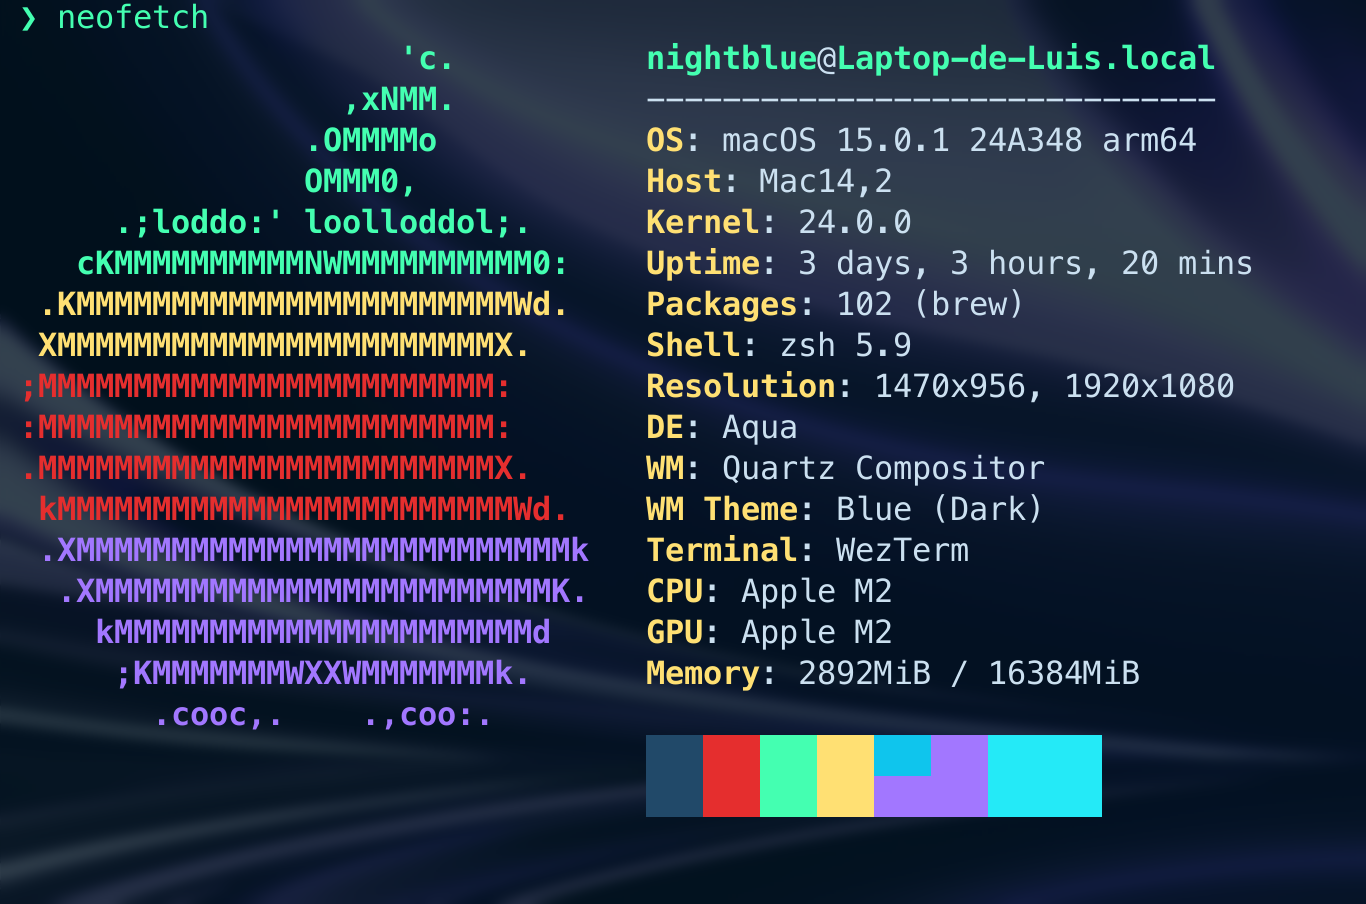
\includegraphics[width=0.7\textwidth]{images/neofetch.png}
    \caption{Detalle del sistema usando el comando \texttt{neofetch}.}
    \label{fig:neofetch}
\end{figure}

\subsection*{Condiciones de Entrada y Parámetros}

Cada experimento fue ejecutado bajo las siguientes condiciones de entrada y parámetros específicos:
\begin{itemize}
    \item \textbf{Cadenas de Entrada:} Se utilizaron cadenas de prueba de diferentes longitudes y combinaciones de caracteres para evaluar el rendimiento de los algoritmos de distancia mínima de edición (alfabeto inglés en letras minúsculas). 
    \item \textbf{Parámetros de Algoritmos:} Los costos para inserción, eliminación, sustitución y transposición fueron establecidos de acuerdo a las especificaciones de los algoritmos.
    \item \textbf{Orden de ejecución de archivos:} Primero se deben crear los archivos de costos (en caso de que no estén creados o se quieran cambiar); luego se debe ejecutar el \verb|main.cpp|, este sobreescribirá los archivos de los resultados y operaciones; por último, ejecutar el archivo Python si se quieren obtener las gráficas.
\end{itemize}

Es importante mecnionar, que esta implementación utiliza la biblioteca \texttt{sys/resource.h} de C++, la cual permite la lectura del consumo de memoria en las operaciones, pero solo está disponible en entornos Linux y Unix. En caso de utilizar un entorno diferente, será necesario eliminar esta funcionalidad en el archivo \textbf{main.cpp}. Esto implicará realizar modificaciones tales como eliminar la función de lectura de memoria del \texttt{main} y omitir la escritura de este dato en el archivo de resultados.



% Autor
% Luis Zegarra Stuardo
% 202073628-6
% Tarea 2 y 3
% Algoritmos y Complejidad 2024-2
\subsection{Dataset (casos de prueba)}
\begin{mdframed}
    \textbf{La extensión máxima para esta sección es de 2 páginas.}
\end{mdframed}

Para los casos de prueba, se decidió no generarlos de manera automática, con el objetivo de mantener control sobre los casos a evaluar y verificar que los algoritmos ejecuten correctamente los pasos necesarios para alcanzar la solución. Los casos de prueba fueron diseñados tomando en cuenta los siguientes escenarios:

\begin{itemize} 
    \item Casos donde las cadenas están vacías: Ejemplos incluyen S1 = $""$ y S2 = $""$, S1 = $"$aaa$"$ y S2 = $""$, \\ 
    y S1 = $""$ y S2 = $"$xyz$"$. 
    \item Casos con caracteres repetidos: Ejemplos incluyen S1 = $"$aabb$"$ y S2 = $"$ab$"$, y S1 = $"$abc$"$ y \\
    S2 = $"$abc$"$. 
    \item Casos donde las transposiciones son necesarias: Ejemplos incluyen S1 = $"$abcd$"$ y S2 = $"$abdc$"$, y \\
    S1 = $"$ab$"$ y S2 = $"$ba$"$. 
    \item Casos variando el largo de las cadenas.
\end{itemize}

Los casos de prueba están almacenados en el archivo \texttt{casos\_prueba.txt}. En este archivo se pueden agregar las líneas que se deseen probar, utilizando el formato ``\texttt{palabra1 palabra2}``. Para representar una cadena vacía, se debe emplear el símbolo de comillas dobles ($""$).

\subsection{Documentación de Casos de Prueba}

A continuación se presentan los casos de prueba utilizados (Figura \ref{fig:teststrings}) para evaluar los algoritmos de distancia de edición. En cada uno se especifican las entradas \( S1 \) y \( S2 \), las operaciones esperadas, el costo total estimado y la justificación de la salida.

\begin{table}[!ht]
    \centering
    \footnotesize
    \begin{tabular}{|c|l|l|p{5cm}|p{4cm}|}
    \hline
    \textbf{Caso de Prueba} & \textbf{Entrada \( S1 \)} & \textbf{Entrada \( S2 \)} & \textbf{Operaciones Esperadas} & \textbf{Costo Total Esperado} \\
    \hline
    1 & $"$abc$"$ & $"$abc$"$ & Ninguna operación. & 0 \\
    2 & $"$ab$"$ & $"$ba$"$ & Transposición de 'a' y 'b'. & Costo transposición \\
    3 & $"$abc$"$ & $"$acb$"$ & Transposición de 'b' y 'c'. & Costo transposición \\
    4 & $"$abcde$"$ & $"$abcde$"$ & Ninguna operación. & 0 \\
    5 & $"$abc$"$ & $"$a$"$ & Eliminación de 'b', Eliminación de 'c'. & 2 * Costo eliminación \\
    6 & $"$abc$"$ & $"$def$"$ & Sustitución de 'a' $\rightarrow$ 'd', 'b' $\rightarrow$ 'e', 'c' $\rightarrow$ 'f'. & 3 * Costo sustitución \\
    7 & $"$abcd$"$ & $"$abdc$"$ & Transposición de 'c' y 'd'. & Costo transposición \\
    8 & $"$aaa$"$ & $"$""$"$ & Eliminación de 'a', 'a', 'a'. & 3 * Costo eliminación \\
    9 & $"$""$"$ & $"$xyz$"$ & Inserción de 'x', 'y', 'z'. & 3 * Costo inserción \\
    10 & $"$""$"$ & $"$""$"$ & Ninguna operación. & 0 \\
    11 & $"$cuadrado$"$ & $"$cuaresma$"$ & Sustitución de 'd' $\rightarrow$ 'r', 'r' $\rightarrow$ 'e', 'a' $\rightarrow$ 's', 'd' $\rightarrow$ 'm', 'o' $\rightarrow$ 'a'. & 5 * Costo sustitución \\
    12 & $"$rodilla$"$ & $"$paella$"$ & Sustitución de 'r' $\rightarrow$ 'p', 'o' $\rightarrow$ 'a', 'd' $\rightarrow$ 'e'. Eliminación de 'i' & 3 * Costo sustitución + 1 * Costo Eliminación\\
    13 & $"$amanda$"$ & $"$ada$"$ & Eliminación de 'm', 'a', 'n'. & 3 * Costo eliminación \\
    \hline
    \end{tabular}
    \caption{Algunos casos de prueba para demostrar operaciones y costo esperado.}
\end{table}
    

\subsubsection{Explicación de Ejecución}

Cada caso ha sido diseñado para cubrir un escenario específico de edición, como inserciones, eliminaciones, sustituciones y transposiciones. A continuación se presenta la justificación por tipo de caso:

\begin{itemize}
    \item \textbf{Igualdad Directa (Casos 1 y 4)}: No requieren cambios, ya que ambas cadenas son idénticas.
    \item \textbf{Transposiciones Necesarias (Casos 2, 3, 7)}: Requieren una transposición para igualar \( S1 \) y \( S2 \), minimizando las operaciones de edición.
    \item \textbf{Inserciones y Eliminaciones (Casos 5, 8, 9, 13)}: Estos casos requieren insertar o eliminar caracteres adicionales en \( S1 \) o \( S2 \) para hacerlas equivalentes.
    \item \textbf{Sustituciones (Casos 6, 11, 12)}: Exigen reemplazar uno o varios caracteres para obtener la cadena deseada.
\end{itemize}

Es importante tener en cuenta que esto es solo una predicción de lo que debería ocurrir, pero pueden existir variaciones. Esto se debe a que la implementación está orientada a encontrar la distancia de edición con costos variables que se generan de manera aleatoria. Por lo tanto, la selección de las operaciones dependerá directamente de los valores con los que se generen los archivos de costos.


\subsection{Resultados}
\textbf{La extensión máxima para esta sección es de 4 páginas.}

\subsubsection{Comprobación de algoritmos}
Primero se detallará el desarrollo para verificar que los algoritmos están correctamente diseñados, proporcionando así resultados correctos. Para esto, se ha utilizado la página web \href{https://es.planetcalc.com/1721/}{PLANETCALC}, la cual cuenta con un apartado para calcular la Distancia de Levenshtein con costos iguales para todas las operaciones. En esta página solo se entrega el resultado, por lo que se comparará este con el resultado obtenido por los algoritmos de Fuerza Bruta y Programación Dinámica.

\begin{table}[H]
    \centering
    \footnotesize
    \begin{tabular}{|c|l|l|l|l|l|}
    \hline
    \textbf{Caso de Prueba} & \textbf{Entrada \( S1 \)} & \textbf{Entrada \( S2 \)} & \textbf{PLANETCALC} & \textbf{Fuerza Bruta} & \textbf{Programación Dinámica} \\
    \hline
    1 & $"$abc$"$ & $"$abc$"$ & 0 & 0 & 0 \\
    2 & $"$ab$"$ & $"$ba$"$ & 1 & 1 & 1 \\
    3 & $"$abc$"$ & $"$acb$"$ & 2 & 1 & 1 \\
    4 & $"$abcde$"$ & $"$abcde$"$ & 0 & 0 & 0 \\
    5 & $"$abc$"$ & $"$a$"$ & 2 & 2 & 2 \\
    6 & $"$abc$"$ & $"$def$"$ & 3 & 3 & 3 \\
    7 & $"$abcd$"$ & $"$abdc$"$ & 1 & 1 & 1 \\
    8 & $"$aaa$"$ & $"$""$"$ & 3 & 3 & 3 \\
    9 & $"$""$"$ & $"$xyz$"$ & 3 & 3 & 3 \\
    10 & $"$""$"$ & $"$""$"$ & 0 & 0 & 0 \\
    11 & $"$cuadrado$"$ & $"$cuaresma$"$ & 5 & 5 & 5 \\
    12 & $"$rodilla$"$ & $"$paella$"$ & 4 & 4 & 4 \\
    13 & $"$amanda$"$ & $"$ada$"$ & 3 & 3 & 3 \\
    \hline
    \end{tabular}
    \caption{Comprobación de la efectividad de los algoritmos con algunos casos de prueba}
    \label{fig:comparacion}
\end{table}

Este paso es solo para verificar que los algoritmos están correctamente diseñados o, al menos, que arrojan el resultado correcto. Para esto, se utiliza el archivo \texttt{costos.cpp}, el cual genera los archivos \texttt{costos} con valor 1 para todas las operaciones, de la siguiente manera:

\begin{itemize}
   \item Contenido de los archivos \texttt{cost\_delete.txt} y \texttt{cost\_insert.txt} so una fila de 26 unos, cada uno representa una letra.
   \item El contenido de los archivos \texttt{cost\_replace.txt} y \texttt{cost\_transpose.txt} son matrices simétrics de \texttt{26x26} que representan el valor de cambiar una letra por otra con un 1. 
\end{itemize}

Se puede observar en el Cuadro \ref{fig:comparacion} que los valores obtenidos son bastante similares, pero esto puede resultar engañoso, ya que la página PLANETCALC utiliza el cálculo original de la Distancia de Levenshtein, donde solo se consideran las operaciones de inserción, eliminación y reemplazo. Es por esto que estas medidas solo se tomaron como referencia para verificar los algoritmos.

\subsubsection{Soluciones encontradas}
Para generar los costos variables, los cuales son requisitos dentro del problema a resolver, se creó el archivo \texttt{random-costos.cpp}, el cual genera los costos asignando un valor aleatorio de 1 a 10 para cada operación. Los costos utilizados pueden verse en el repositorio de Github, aquí están los enlaces:

\begin{itemize}
    \begin{minipage}{0.5\textwidth}
        \item \href{https://github.com/luphin/Tarea2y3Algoritmos-FB-PD/blob/main/codigos/cost_delete.txt}{delete}
        \item \href{https://github.com/luphin/Tarea2y3Algoritmos-FB-PD/blob/main/codigos/cost_insert.txt}{insert}
    \end{minipage}%
    \begin{minipage}{0.5\textwidth}
        \item \href{https://github.com/luphin/Tarea2y3Algoritmos-FB-PD/blob/main/codigos/cost_replace.txt}{replace}
        \item \href{https://github.com/luphin/Tarea2y3Algoritmos-FB-PD/blob/main/codigos/cost_transpose.txt}{transpose}
    \end{minipage}
\end{itemize}


Al ejecutar el \verb|main.cpp| con estos costos, los resultados obtenidos se pueden evidenciar en el archivo \verb|resultados.txt|, en el cual se encuentra que:

\begin{table}[H]
    \centering
    \footnotesize
    \begin{tabular}{|c|l|l|l|l|}
    \hline
    \textbf{Caso de Prueba} & \textbf{Entrada \( S1 \)} & \textbf{Entrada \( S2 \)} & \textbf{Distancia (FB)} & \textbf{Distancia (PD)} \\
    \hline
    1 & $"$abc$"$ & $"$abc$"$ & 0 & 0 \\
    2 & $"$ab$"$ & $"$ba$"$ & 3 & 3 \\
    3 & $"$abc$"$ & $"$acb$"$ & 2 & 2 \\
    4 & $"$abcde$"$ & $"$abcde$"$ & 0 & 0 \\
    5 & $"$abc$"$ & $"$a$"$ & 4 & 4 \\
    6 & $"$abc$"$ & $"$def$"$ & 14 & 14 \\
    7 & $"$abcd$"$ & $"$abdc$"$ & 2 & 2 \\
    8 & $"$aaa$"$ & $"$""$"$ & 6 & 6 \\
    9 & $"$""$"$ & $"$xyz$"$ & 15 & 15 \\
    10 & $"$""$"$ & $"$""$"$ & 0 & 0 \\
    11 & $"$cuadrado$"$ & $"$cuaresma$"$ & 15 & 15 \\
    12 & $"$rodilla$"$ & $"$paella$"$ & 20 & 20 \\
    13 & $"$amanda$"$ & $"$ada$"$ & 13 & 13 \\
    \hline
    \end{tabular}
    \caption{Comprobación }
    \label{fig:resultados}
\end{table}

\begin{figure}[H]
    \centering
    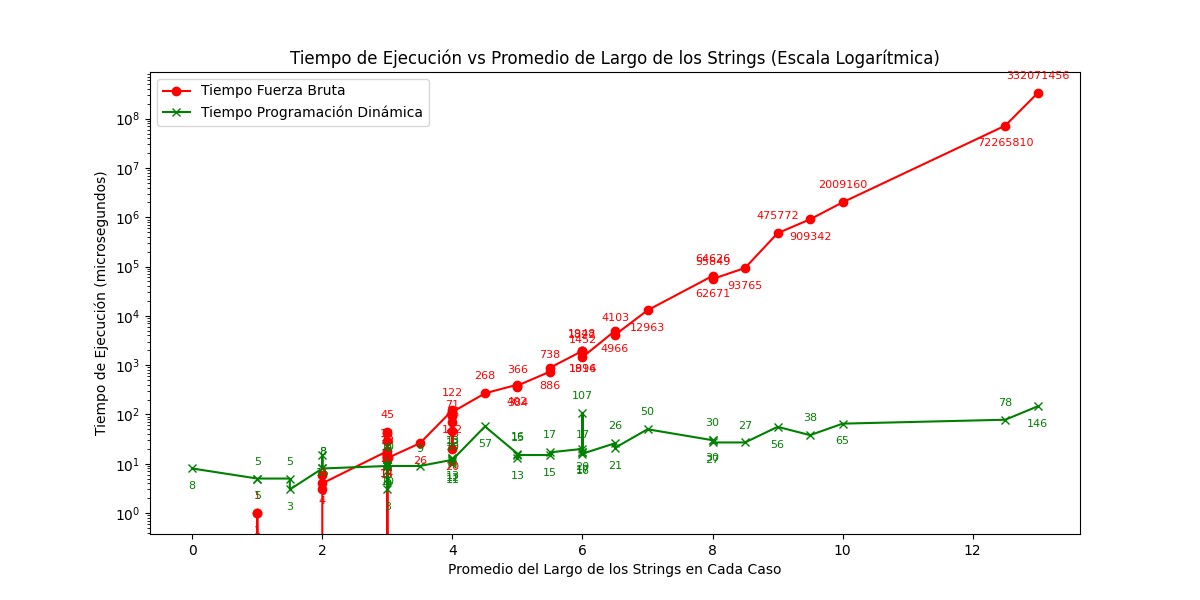
\includegraphics[width=1\textwidth]{images/Figure_1.png}
    \caption{Gráfica obtenida con los resultados de las pruebas.}
    \label{fig:tiempo}
\end{figure}
\begin{figure}[H]
    \centering
    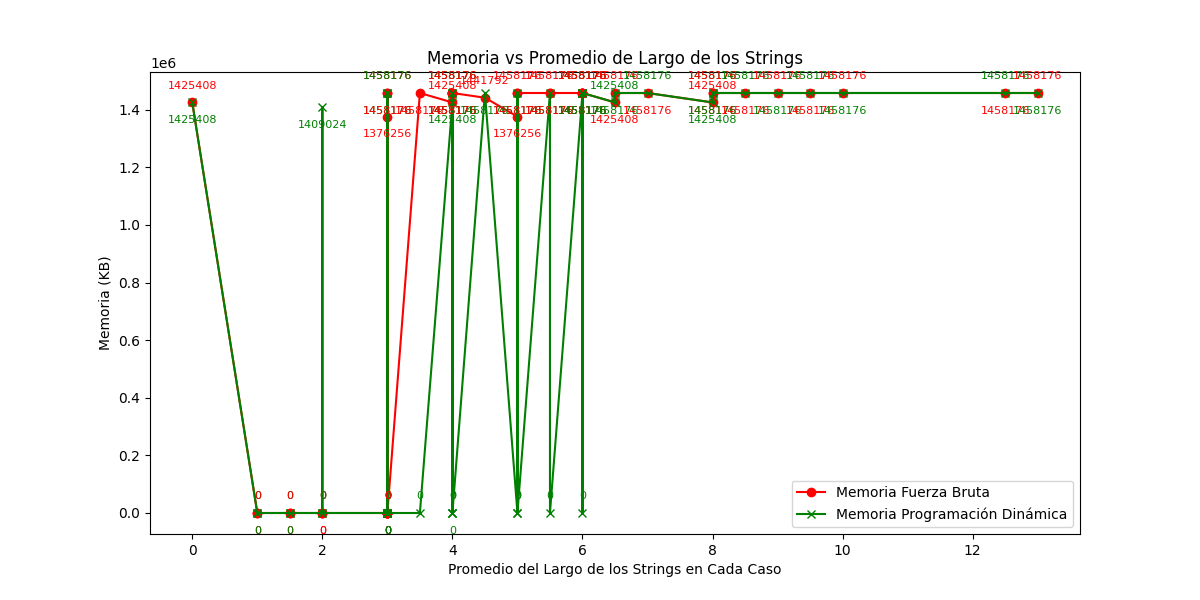
\includegraphics[width=1\textwidth]{images/Figure_2.png}
    \caption{Gráfica obtenida con resultados de las pruebas.}
    \label{fig:memoria}
\end{figure}

La Figura \ref{fig:tiempo} es originada en base a los resultados de los casos de prueba que son anotados en \href{https://github.com/luphin/Tarea2y3Algoritmos-FB-PD/blob/main/codigos/resultados.txt}{resultados.txt}, se puede ver el comportamiento de los algortimos en base al tiempo que demoran dependiendo de la longitud de las cadenas, tambien influye como la cadena esta estructurada. A medida que aumenta el promedio de la suma de largos de las cadenas el tiempo de ejecucion aumenta en mayor porporcion para el algoritmo de Fuerza bruta, en relacion al cambio más controlado que se puede ver en el algoritmos de Programación diámica. Tambien se trato de obtener la memoria utilizada por cada una de las funciones para resolver el problema, esto mediante un hilo que se ejecutara en paralelo con la ejecuion del archivo \texttt{main.cpp} de esta forma ir consultando la memoria utilizada cada 50 milisegundos y esta almacenandola en una variable global (no se ejecuto ningun programa más mientras estaba en ejecución main) se obtuvo lo graficado en la Figura \ref{fig:memoria}.


\newpage
\section{Conclusiones}
Los resultados obtenidos a partir de las simulaciones demuestran de manera clara la superioridad del algoritmo de Programación Dinámica frente al de Fuerza Bruta en cuanto al tiempo de ejecución. A medida que el tamaño de las cadenas de entrada aumenta, el algoritmo de Programación Dinámica muestra una eficiencia notablemente mayor en términos de tiempo, lo que valida su eficacia para resolver el problema planteado.

En cuanto al análisis de la memoria, los resultados no son concluyentes debido a la deficiencia en la implementación de la medición de memoria. Las variaciones observadas en el uso de memoria pueden atribuirse tanto a limitaciones del compilador, que optimiza el uso de memoria en ciertos casos, como a posibles fallos en la implementación de los registros dentro del archivo \texttt{operaciones.txt}, lo cual limitó la revición sobre los pasos que siguiieron cada algoritmo para encontrar la solución, ya que, se registraron gran parte de las reviciones realizadas y no solos las que aportaban en el cálculo de la solución final.

A pesar de estas dificultades, el análisis realizado confirma que ambos algoritmos son adecuados para resolver el problema de calcular la menor distancia de edición con costos variables, aunque la obtención de los pasos intermedios de cada algoritmo no fue posible debido a los problemas con la implementación del manejo de registros. Estos resultados contribuyen a una mejor comprensión de las ventajas y limitaciones de los algoritmos en el contexto de la distancia de edición con costos variables, destacando la importancia de una implementación precisa para obtener métricas confiables.



% Autor
% Luis Zegarra Stuardo
% 202073628-6
% Tarea 2 y 3
% Algoritmos y Complejidad 2024-2

\newpage

\section{Condiciones de entrega}
% Condiciones generales de tareas de Algoritmos y Complejidad, 20231
  \begin{itemize}
  \item
    La tarea se realizará \tca{individualmente}
    (esto es grupos de una persona),
    sin excepciones.
  \item
    La entrega debe realizarse vía \url{http://aula.usm.cl}
    en un \tca{tarball} en el área designada al efecto,
    en el formato \tca{\texttt{tarea-\tnum-{rol}.tar.gz}}
    (\texttt{rol} con dígito verificador y sin guión).

    Dicho \tca{tarball} debe contener las fuentes en \LaTeXe{}
    (al menos \tca{\texttt{tarea-\tnum.tex}})
    de la parte escrita de su entrega,
    además de un archivo \tca{\texttt{tarea-\tnum.pdf}},
    correspondiente a la compilación de esas fuentes.
  \item Si se utiliza algún código, idea, o contenido extraído de otra fuente, este \textbf{debe} ser citado en el lugar exacto donde se utilice, en lugar de mencionarlo al final del informe. 
  \item
    Asegúrese que todas sus entregas tengan sus datos completos:
    número de la tarea, ramo, semestre, nombre y rol.
    Puede incluirlas como comentarios en sus fuentes \LaTeX{}
    (en \TeX{} comentarios son desde \% hasta el final de la línea)
    o en posibles programas.
    Anótese como autor de los textos.
 
  \item
    Si usa material adicional al discutido en clases,
    detállelo.
    Agregue información suficiente para ubicar ese material
    (en caso de no tratarse de discusiones con compañeros de curso
     u otras personas).
  \item No modifique \texttt{preamble.tex}, \texttt{tarea\_main.tex}, \texttt{condiciones.tex}, estructura de directorios, nombres de archivos, configuración del documento, etc. Sólo agregue texto, imágenes, tablas, código, etc. En el códigos funte de su informe, no agregue paquetes, ni archivos .tex (a excepción de que agregue archivos en \texttt{/tikz}, donde puede agregar archivos .tex con las fuentes de gráficos en \texttt{TikZ}).

\ifprograms
  \item
    Su programa ejecutable debe llamarse \tca{\texttt{tarea\tnum}},
    de haber varias preguntas solicitando programas,
    estos deben llamarse usando el número de la pregunta,
    como \tca{\texttt{tarea\tnum-1}},
    \tca{\texttt{tarea\tnum-2}},
    etc.
    Si hay programas compilados, con en este caso,
    incluya una \tca{\texttt{Makefile}}
    que efectúe las compilaciones correspondientes.

    Los programas se evalúan según que tan claros
    (bien escritos)
    son, si se compilan y ejecutan sin errores o advertencias según corresponda.
    Parte del puntaje es por ejecución correcta con casos de prueba.
    Si el programa no se ciñe a los requerimientos de entrada y salida,
    la nota respectiva es cero.
\fi    
  \item
    %La entrega debe realizarse dentro del plazo indicado en \url{http://aula.usm.cl}:
    La fecha límite de entrega es el día \tca{10 de noviembre de 2024}.

    \begin{center}
        \Large{
          \textbf{NO SE ACEPTARÁN TAREAS FUERA DE PLAZO}.
        }
        \normalsize
    \end{center}
     
    
  \item
    Nos reservamos el derecho de llamar a interrogación
    sobre algunas de las tareas entregadas.
    En tal caso,
    la nota de la tarea será la obtenida en la interrogación.
    \begin{center}
      \Large{
        \textbf{NO PRESENTARSE A UN LLAMADO A INTERROGACIÓN SIN JUSTIFICACIÓN PREVIA SIGNIFICA AUTOMÁTICAMENTE NOTA 0.}
      }
    \end{center}
    
  \end{itemize}

%%% Local Variables:
%%% mode: latex
%%% ispell-local-dictionary: "spanish"
%%% End:

  
% LocalWords:  tarball tar gz pdf min entregable Makefile puntaje
% LocalWords:  Moodle

\newpage
\appendix


\section{Apéndice 1}
\begin{figure}[H]
    \centering
    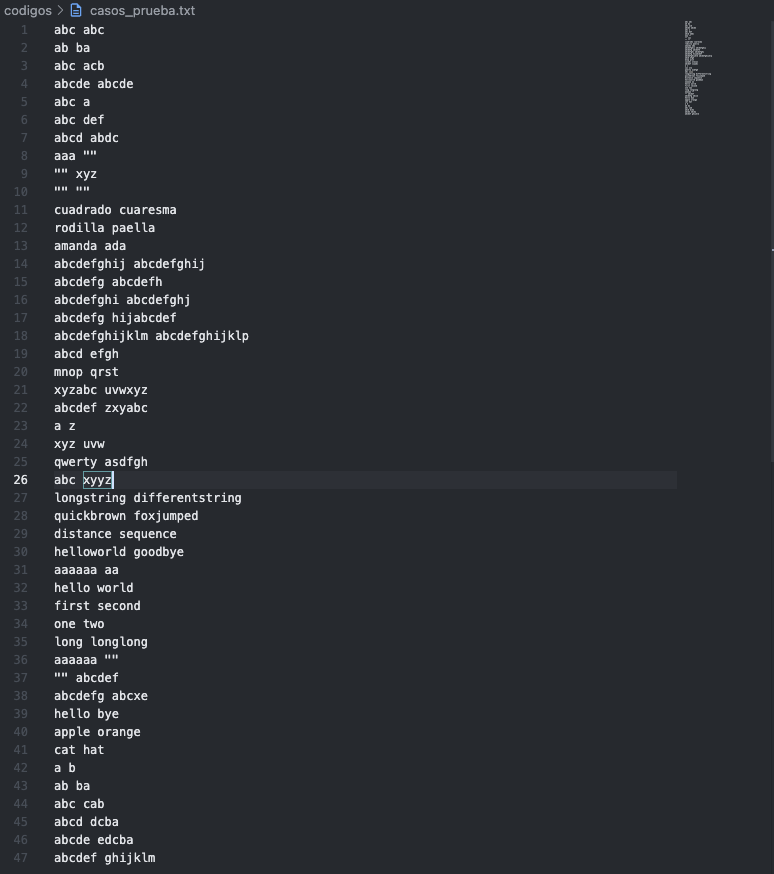
\includegraphics[width=0.8\textwidth]{images/teststrings.png}
    \caption{Casos de prueba}
    \label{fig:teststrings}
\end{figure}
\printbibliography

\end{document}


